\subsection{Analyse de paquets}

Afin de pouvoir étudier finement les échanges de paquets entre les cartes, notre tuteur nous a fourni une carte spécialisée dans la capture de trames, la CC 2531 (\cref{cc2531}).
Elle est équipée d’un port USB de type A qui permet de la brancher directement sur un ordinateur en vue de l’utiliser avec un logiciel d’analyse.

\begin{figure}[H]
\centering
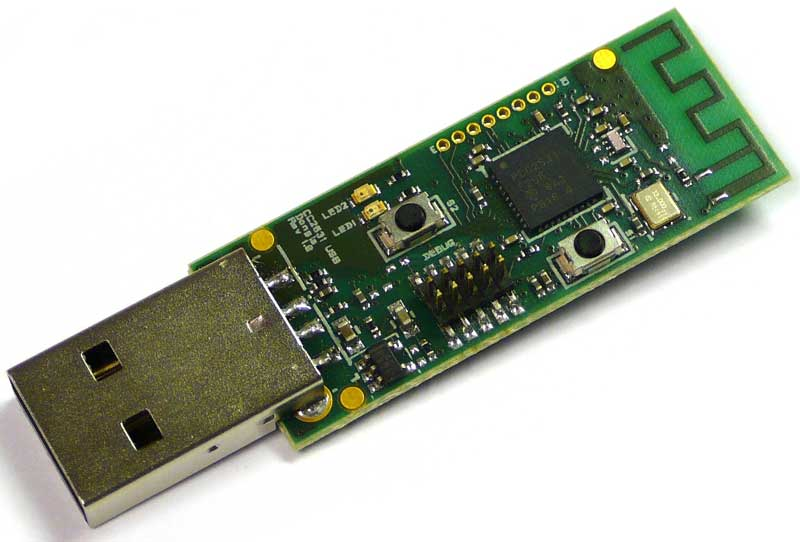
\includegraphics[width=8cm]{\rpDossier/images/cc2531.jpg}
\caption{Carte CC 2531 pour la capture de trames}
\label{cc2531}
\end{figure}

Nous avons utilisé pour l’analyse le logiciel fourni par TI, \emph{SmartRF Packet Sniffer}.
Celui-ci ne fournissant pas de décodage spécifique à 6LoWPAN, nous l’avons utilisé directement au niveau 802.15.4.

\emph{SmartRF Packet Sniffer} ne permet pas une analyse simultanée de tous les canaux disponibles.
Cela impose de parcourir à la main toutes celles disponibles lorsqu’on ne dispose pas d’un moyen aisé pour déterminer celui qui est utilisé.
Malgré un tel parcours, nous n’avons pas pu voir de trames lors de nos premières utilisations (à l’exception d’erreurs sur le canal 1).
Pensant qu’il y avait un problème de fonctionnement, nous avons laisé de côté l’analyse des paquets pour nous concentrer sur le développement du dispositif de démonstration.

Nous avons cependant pu par la suite trouver le canal lors d’une rencontre avec notre tuteur, qui nous a par ailleurs conseillé de commencer préférentiellement par les derniers canaux, plus probables dans un environnement avec de nombreuses communications Wi-Fi comme celui où nous travaillons.

Nous avons à cette occasion découvert que les messages envoyés par les cartes étaient dupliqués de nombreuses fois : certaines trames sont envoyées une vingtaine de fois.

\todo[explications ?]

